\documentclass[ignorenonframetext,10pt]{beamer}
%\documentclass[paper=a4,12pt,version=last,landscape]{scrartcl}

%\usepackage[latin1]{inputenc}
\usepackage[english]{babel}
\usepackage{amsmath,amssymb}
\usepackage{multimedia}
\usepackage{alltt}
\usepackage{multirow}
\usepackage{textcomp}
\usepackage[footnotesize]{subfigure}
\usepackage{graphicx}


\usepackage{pgfplots}
\pgfplotsset{width=7cm,compat=1.3}% <-- moves axis labels near ticklabels (respects tick label widths)
\usepackage{pgfplotstable}



%\usetheme{Berlin}
\usetheme{Darmstadt}
\useoutertheme[subsection=false]{miniframes}
\useoutertheme{smoothbars}
\usefonttheme{structurebold}
%\setbeamertemplate{navigation symbols}{}
\setbeamercovered{invisible}


\title{Helices indices of RNAs}
\author{\large Jiabin~Huang}
\date{\today}

\institute[ExpBI]{\normalsize
Genetics \& Experimental Bioinformatics\\
University Freiburg\\
Institute of Biology III}
  



\begin{document}

\frame{\maketitle}

% frame 2
\begin{frame}
\frametitle{Outline}
   \begin{itemize}
   \item an overview of RNA secondary structure elements and a classical RNA secondary structure prediction algorithm
   \item introducing concept of abstract shapes  
   \item basic ideas about the helices indices
   \item outlook            
   \end{itemize}
\end{frame}


% PART 1: RNA secondary structure elements and classical algorithm
\section{RNA secondary structure elements and classical algorithm}
% frame 3  
\begin{frame}
\frametitle{Secondary structure elements of RNA}  
\begin{figure}
  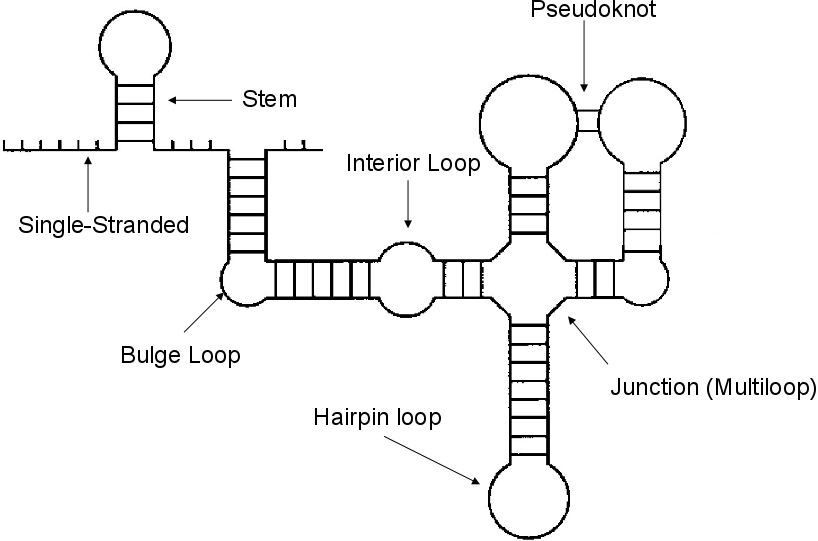
\includegraphics[scale=0.35]{images/RNA_components.jpg} 
  \caption{Secondary structure elements of RNA, all double stranded regions are also called as ''helices''}
\end{figure}
\end{frame}


% frame 4
\begin{frame}
\frametitle{\large Classical secondary structure algorithms (Zuker 1981)}
  \begin{block}{facts about Zuker algorithm}
    \begin{itemize}
    \item first described by Zuker and Stiegler in 1981
    \item basic idea: 
    \begin{enumerate}
      \item a RNA sequence can be folded into many different secondary structure
      \item for every secondary structure, we can calculate a free energy
      \item after that, the algorithm choose the structure with the minimum free energy
    \end{enumerate}
    \item the runtime is $O(n^3)$
    \item can get only one solution
    \end{itemize}
  \end{block}
\end{frame}


% frame 5
\begin{frame}
\frametitle{Free energy computation example}  
\begin{figure}
  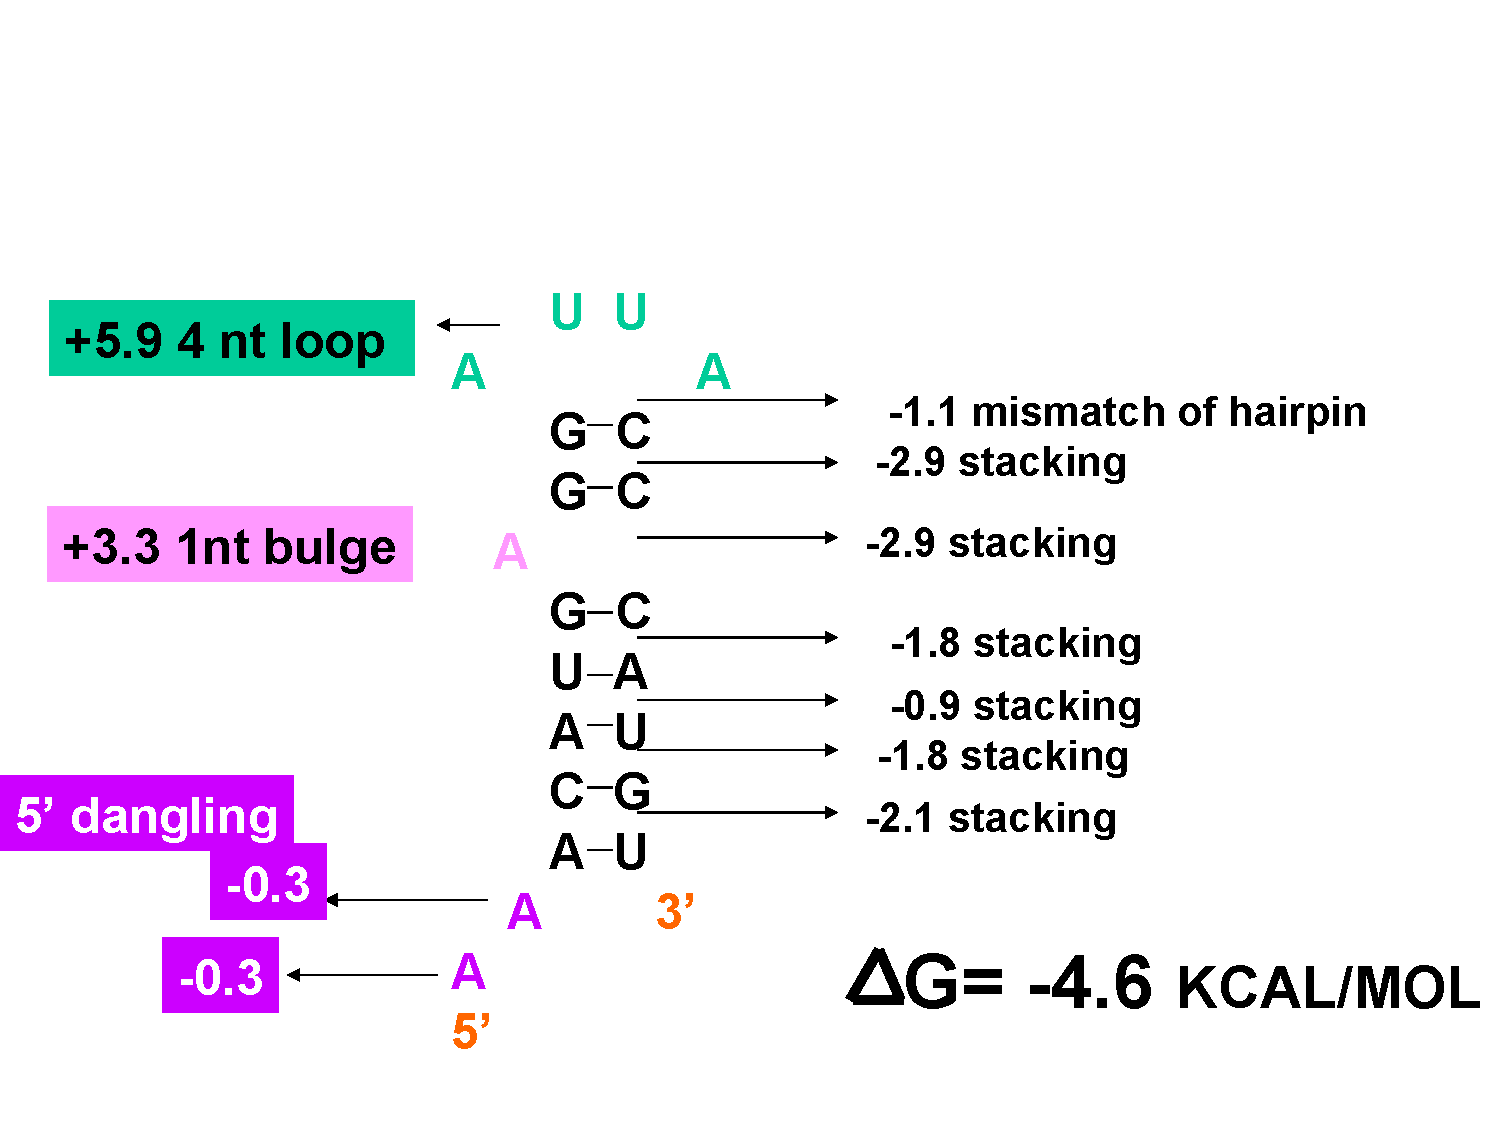
\includegraphics[scale=0.4]{images/mfe_example.pdf} 
\end{figure}
\end{frame}


% frame 6
\begin{frame}
\frametitle{energy landscape}
\begin{figure}
  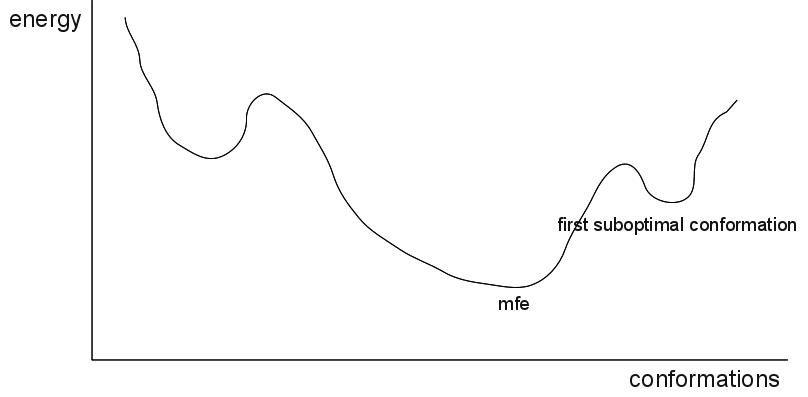
\includegraphics[scale=0.4]{images/energy_landscape_simple.jpg}
\end{figure}
\end{frame}


% frame 7  
\begin{frame}
\frametitle{Suboptimal structures}
  %\begin{block}
  \begin{itemize} 
    \item the native structure is not always the one with the lowest predicted free energy.
    \item but it must not be far away from the mfe point and it is normally a local minimum
    \item how to find the native structure: enumerate all suboptimal structures within a given energy range
  \end{itemize}
  %\end{block}   
\end{frame}


% frame 8
\begin{frame}
\frametitle{energy landscape setting a range}  
\begin{figure}
  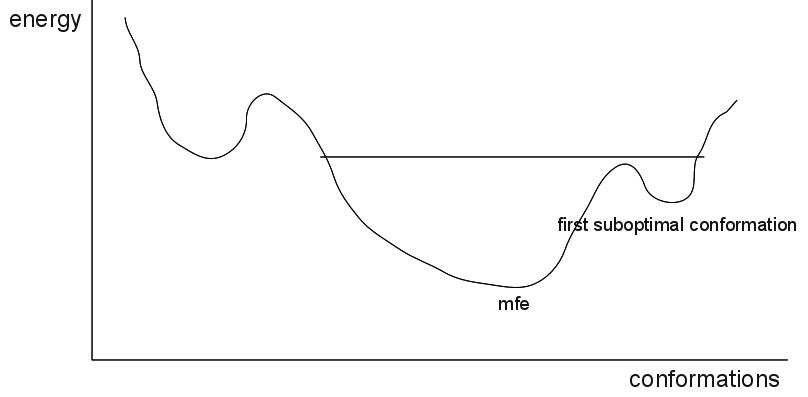
\includegraphics[scale=0.4]{images/energy_landscape_area.jpg} 
\end{figure}
but the number of suboptimal structures grows exponentially with the energy range considered.
\end{frame}


% PART 2: abstract shapes
\section{abstract shapes}
% frame 9
\begin{frame}
\frametitle{Introducing abstract shape}
    Solution: further classify secondary structures space within the energy range with different approaches.
    \begin{itemize} 
    \item abstract shape is one approach in this direction
    \item developed by Giegerich and Voss
    \item intial idea:
    \begin{enumerate}
      \item the user is usually only interested in structures that show fundamental differences
      \item small changes, such as additional base pairs or changing bulge loops are of minor significance
    \end{enumerate}
    \item central to this approach: do not care about all details of the structures and abstract from some types secondary structure elements and length of them
    \item each shape has a representative structure called shrep (with minimum free energy within the shape class)
    \end{itemize}
\end{frame}


% frame 10
\begin{frame}
\frametitle{Abstract shapes, energy range: 5 kcal/mol}  
\begin{figure}
  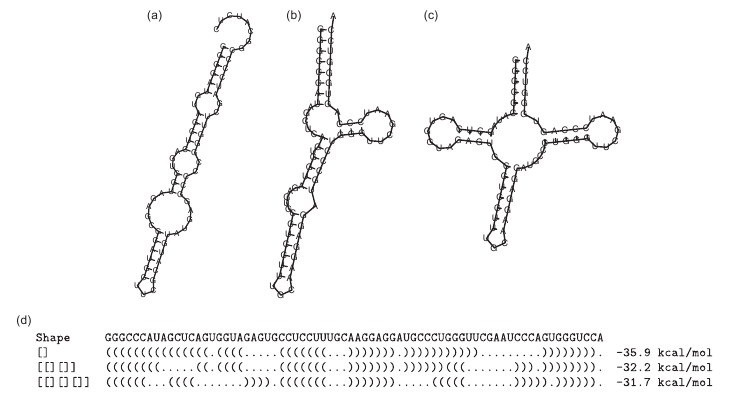
\includegraphics[scale=0.6]{images/shapes_example.jpg} 
\end{figure}
\end{frame}


% PART 3: helices indices
\section{helices indices}
% frame 11
\frametitle{Drawback of abstract shape}
\begin{frame}
\frametitle{Drawback of abstract shape}
   \begin{block}{\small Drawback of abstract shape}
   \begin{itemize} 
   \item abstract shape is position independent
   \end{itemize}
   \end{block}
   \begin{block}{\small Consequence of the drawback}
   \begin{figure}
     \item make the current implementation of shape abstraction unsuitable for the analysis of folding landscapes in a detailed fashion
   \end{figure}
   \end{block}  
   \begin{block}{\small Example}
   \begin{figure}
     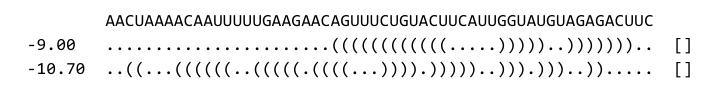
\includegraphics[scale=0.55]{images/drawback_1.jpg} 
   \end{figure}
   \end{block}      
\end{frame}


% frame 12
\begin{frame}
\frametitle{develop a new structure abstraction: helices indices}
    The straightforward idea to overcome the drawback is to develop a new structure abstraction that includes the information of positions of helices
    \begin{block}{Which secondary structure element should be recorded?}
    \begin{itemize} 
    \item hairpin loop
    \item multiloop
    \item bulge or internal loops
    \item any combinations of them
    \end{itemize}
    \end{block}
    \begin{block}{Which position of this element should be recorded?}
    \begin{itemize} 
    \item i
    \item j   
    \item i,j
    \item (i+j)/2
    \end{itemize}    
    \end{block}
\end{frame}


% frame 13
% frame landscape
\begin{frame}
\frametitle{helices positions example}  
\begin{figure}
  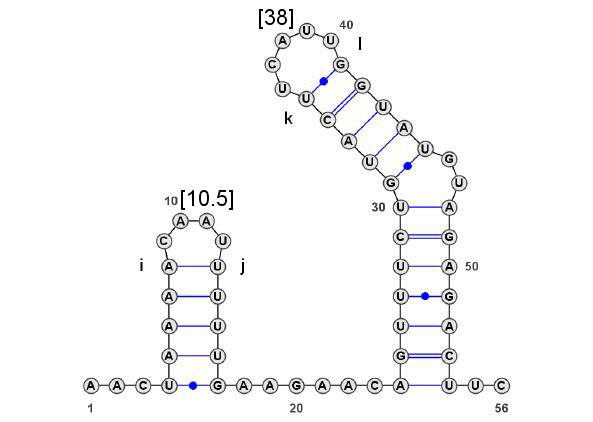
\includegraphics[scale=0.5]{images/helices_position.jpg} 
  \caption{The structure is composed of two helices which are closed by hairpin
  loops (i,j) and (k,l), respectively. The positions are: i=8, j=13, k=35 and
  l=41. Thus, this structure would be abstracted to [10.5,38]}
\end{figure}
\end{frame}

% frame 14
\begin{frame}[fragile]
  Output from the first version of helices indices
  \begin{block}{\tiny Helices indices, energy range: 10 kcal/mol}
  %\begin{alltt}     %[fontsize=\small] 
  \tiny
  \begin{verbatim}
     AACUAAAACAAUUUUUGAAGAACAGUUUCUGUACUUCAUUGGUAUGUAGAGACUUC
-10.7..((...((((((..(((((.((((...)))).)))))..))).)))..))..... [27] *
-9.0 .......................((((((((((((.....)))))..))))))).. [38] *
-7.7 ...(((((....)))))......((((((((((((.....)))))..))))))).. [10.5,38]
-7.4 ........(((...)))......((((((((((((.....)))))..))))))).. [13,38]
-7.1 ..........(((..(((((.((((...)))).)))))..)))..((....))... [27,49.5]
-6.7 .......((((((..(((((.((((...)))).)))))..))).))).((....)) [27,52.5]
-6.7 ..((..((......))..))...((((((((((((.....)))))..))))))).. [11.5,38]
-6.6 ..((.(((.....)))..))...((((((((((((.....)))))..))))))).. [11,38]
-6.5 ...............(((((.((((...)))).)))))..(((........))).. [27,47.5]
                    ...
-2.4 .....((...(((..(((((.((((...)))).)))))..)))..((....)))). [27,49.5,30.5m]
-2.4 ..(((((....))).(((((.((((...)))).)))))...........))..... [9.5,27,27m]
-2.4 .......................((((((((((......)).....)))))))).. [36.5]
-2.4 ...............(((((.((((...)))).)))))((..........)).... [27,45.5]
-2.4 .......................((((((((...((....))....)))))))).. [38.5]
-2.3 .((((.((....)).(((((.((((...)))).))))).))))..((....))... [10.5,27,22.5m,49.5]
-2.3 ....((....(((..(((((.((((...)))).)))))..)))..((....)))). [27,49.5,30m]
-2.3 ..((.(((.....)))((((.((((...)))).))))............))..... [11,27,27m]
-2.3 ................((((..(((...)))((((.....))))........)))) [27,38,36.5m] *
                    ...
-0.7 ..((...........(((((.((((...)))).))))).((...))...))..... [27,43,27m]
-0.7 ....(((....))).........(((((((..((...........))))))))).. [9.5,40]
-0.7 .........((.(((....)))..(((((((((((.....)))))..)))))))). [17.5,38,32.5m]
-0.7 .((((.((....)).(((((.((((...)))).))))).)))).....((....)) [10.5,27,22.5m,52.5]
-0.7 ....((((...))))........(((((((..((...........))))))))).. [10,40]
-0.7 ((.........))..(((((.((((...)))).)))))..(((........))).. [7,27,47.5]
-0.7 ................((((.....)))).((.((..((......))..))))... [23,42.5]
-0.7 ........((((......((((....)))).......))))....((....))... [24.5,49.5]
-0.7 ..((....(((...))).............(((((.....)))))....))..... [13,38,27m]
-0.7 ..(((.......(((....)))........(((((.....))))).)))....... [17.5,38,26m]
-0.7 ....((.........((.....))(((((((((((.....)))))..)))))))). [20,38,30m]                    
  \end{verbatim} 
  %\end{alltt}
  \end{block}
\end{frame}

\normalsize
% frame 15: energy barrier
\begin{frame}
\frametitle{energy barrier}  
\begin{figure}
  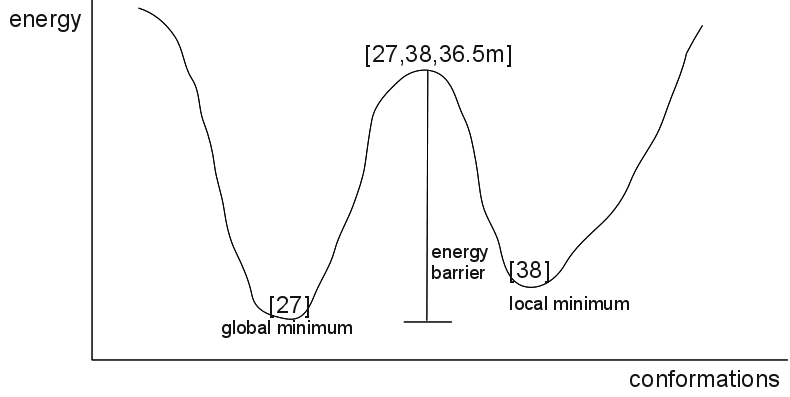
\includegraphics[scale=0.4]{images/energy_barrier.jpg} 
\end{figure}
\end{frame}

% frame 16
\begin{frame}
\frametitle{Problem}
  \small
  %Although the helices space grows considerably slower than structure space, but
  %it is still exponential

  %Growth of structure, helix and shape space 
  The helices indices space grows a lot faster than the abstract shapes space
  \normalsize
  \begin{block}{\tiny Comparison of helices indices space with abstract shapes space}
  %\begin{figure}
    \centering
	\begin{tikzpicture}[scale=0.7]
		%\begin{semilogyaxis}[xlabel=Index,ylabel=Value]
		%\addplot gnuplot[color=blue,mark=*]{1.2196*(x**(-1.5))*(2.6180**x)}; 
		%\end{semilogyaxis}
		\begin{semilogyaxis}[legend style={font=\small},xlabel={Sequence
         length},ylabel={Nr. of helices indices/abstract shapes},width=\textwidth,legend style={nodes=right},
         legend pos= north west]
     
        
         %\addplot+[only marks,mark=+]
         %table[x=X,y=Y]{/home/jiabin/workspace/RNAHeliCes/scripts/estimate_exponent_RNAsubopt.txt};
         %\addlegendentry{Structures}         
         %\addplot table[x=X,y={create col/linear
         %regression={y=Y}}]{/home/jiabin/workspace/RNAHeliCes/scripts/estimate_exponent_RNAsubopt.txt};
         %\addlegendentry{$0.33 \cdot x -3.24$}
         
         
         \addplot+[only marks,mark=-]
         table[x=X,y=Y]{/home/jiabin/workspace/RNAHeliCes/scripts/estimate_exponent_RNAhelix.txt};
         \addlegendentry{Helices}         
         \addplot table[x=X,y={create col/linear
         regression={y=Y}}]{/home/jiabin/workspace/RNAHeliCes/scripts/estimate_exponent_RNAhelix.txt};
         \addlegendentry{$0.18 \cdot x -1.42$} 
 
         \addplot+[only marks,mark=x]
         table[x=X,y=Y]{/home/jiabin/workspace/RNAHeliCes/scripts/estimate_exponent_RNAshapes_5.txt};
         \addlegendentry{Shapes}                   
         \addplot table[x=X,y={create col/linear
         regression={y=Y}}]{/home/jiabin/workspace/RNAHeliCes/scripts/estimate_exponent_RNAshapes_5.txt};                 
         \addlegendentry{
$\pgfmathprintnumber{\pgfplotstableregressiona} \cdot x
\pgfmathprintnumber[print sign]{\pgfplotstableregressionb}$}
         
               
        
        %\addlegendentry{Legenden Eintrag};
        \end{semilogyaxis} 
	\end{tikzpicture}
	%\caption{Growth of structure, helix and shape space}	
  %\end{figure}	
  \end{block}
\end{frame}

% frame 17
\begin{frame}
\frametitle{Solution of the problem}
  \small
  One of the solution: we can limit the helices space by setting an energy range on
  it
  \normalsize
  \begin{block}{\tiny Comparison of helices indices space setting different energy ranges}     
    \centering
	\begin{tikzpicture}[scale=0.7]
		%\begin{semilogyaxis}[xlabel=Index,ylabel=Value]
		%\addplot gnuplot[color=blue,mark=*]{1.2196*(x**(-1.5))*(2.6180**x)}; 
		%\end{semilogyaxis}
		\begin{semilogyaxis}[legend style={font=\tiny},xlabel={Sequence
         length},ylabel={Nr. of helices indices},width=\textwidth,legend
         style={nodes=right}, legend pos= north west]

         \addplot+[only marks,mark=-]
         table[x=X,y=Y]{/home/jiabin/workspace/RNAHeliCes/scripts/estimate_exponent_RNAhelix.txt};
         \addlegendentry{energy range unlimited}
         \addplot table[x=X,y={create col/linear
         regression={y=Y}}]{/home/jiabin/workspace/RNAHeliCes/scripts/estimate_exponent_RNAhelix.txt};
         \addlegendentry{$0.18 \cdot x -1.42$} 

          \addplot+[only marks,mark=x]
          table[x=X,y=Y]{/home/jiabin/workspace/RNAHeliCes/scripts/estimate_exponent_RNAhelix_5_20kcal.txt};
          \addlegendentry{energy range 20kcal/mol}
          \addplot table[x=X,y={create col/linear
          regression={y=Y}}]{/home/jiabin/workspace/RNAHeliCes/scripts/estimate_exponent_RNAhelix_5_20kcal.txt}; 
          \addlegendentry{$0.12 \cdot x +0.44$} 
       
          \addplot+[only marks,mark=x]
          table[x=X,y=Y]{/home/jiabin/workspace/RNAHeliCes/scripts/estimate_exponent_RNAhelix_5_15kcal.txt};
          \addlegendentry{energy range 15kcal/mol}
          \addplot table[x=X,y={create col/linear
          regression={y=Y}}]{/home/jiabin/workspace/RNAHeliCes/scripts/estimate_exponent_RNAhelix_5_15kcal.txt};
          \addlegendentry{$0.0904 \cdot x +1.23$} 

          \addplot+[only marks,mark=x]
          table[x=X,y=Y]{/home/jiabin/workspace/RNAHeliCes/scripts/estimate_exponent_RNAhelix_5_10kcal.txt};
          \addlegendentry{energy range 10kcal/mol}
          \addplot table[x=X,y={create col/linear
          regression={y=Y}}]{/home/jiabin/workspace/RNAHeliCes/scripts/estimate_exponent_RNAhelix_5_10kcal.txt};
          \addlegendentry{$0.0602 \cdot x +1.43$}      
                                        
          \addplot+[only marks,mark=x]
          table[x=X,y=Y]{/home/jiabin/workspace/RNAHeliCes/scripts/estimate_exponent_RNAhelix_5_5kcal.txt};
          \addlegendentry{energy range 5kcal/mol}
          \addplot table[x=X,y={create col/linear
          regression={y=Y}}]{/home/jiabin/workspace/RNAHeliCes/scripts/estimate_exponent_RNAhelix_5_5kcal.txt};
          \addlegendentry{$0.0366 \cdot x +0.7$} 
     
                            
%           \addlegendentry{
%  $\pgfmathprintnumber{\pgfplotstableregressiona} \cdot x
%  \pgfmathprintnumber[print sign]{\pgfplotstableregressionb}$}
         
               
        
        %\addlegendentry{Legenden Eintrag};
        \end{semilogyaxis} 
	\end{tikzpicture}
  \end{block}	
\end{frame}


% PART 4: outlook  
\section{outlook} 
% frame 18
\begin{frame}
\frametitle{Outlook}
    \begin{itemize} 
    \item develop a new structure abstraction (helices indices)
    \item implement a software based on the idea
    \item the software will be evaluated by benchmark program
    \item design a RNA class predictor
    \end{itemize}
\end{frame}


% frame 19
\begin{frame}
\frametitle{End}
   \begin{itemize} 
   \item Thanks a lot for your attention !
   \item Questions ?
   \end{itemize}
\end{frame}


\end{document}
